\documentclass{article}

% if you need to pass options to natbib, use, e.g.:
%     \PassOptionsToPackage{numbers, compress}{natbib}
% before loading neurips_2026

% The authors should use one of these tracks.
% Before accepting by the NeurIPS conference, select one of the options below.
% 0. "default" for submission
\usepackage[final]{neurips_2026}
% the "default" option is equal to the "main" option, which is used for the Main Track with double-blind reviewing.
% 1. "main" option is used for the Main Track
%  \usepackage[main]{neurips_2026}
% 2. "position" option is used for the Position Paper Track
%  \usepackage[position]{neurips_2026}
% 3. "eandd" option is used for the Evaluations & Datasets Track
 % \usepackage[eandd]{neurips_2026}
 % if you want to opt-in for a de-anomymized submission (not recommended, but OK):
 %\usepackage[eandd, nonanonymous]{neurips_2026}
% 4. "creativeai" option is used for the Creative AI Track
%  \usepackage[creativeai]{neurips_2026}
% 5. "sglblindworkshop" option is used for the Workshop with single-blind reviewing
 % \usepackage[sglblindworkshop]{neurips_2026}
% 6. "dblblindworkshop" option is used for the Workshop with double-blind reviewing
%  \usepackage[dblblindworkshop]{neurips_2026}

% After being accepted, the authors should add "final" behind the track to compile a camera-ready version.
% 1. Main Track
 % \usepackage[main, final]{neurips_2026}
% 2. Position Paper Track
%  \usepackage[position, final]{neurips_2026}
% 3. Evaluations & Datasets Track
 % \usepackage[eandd, final]{neurips_2026}
% 4. Creative AI Track
%  \usepackage[creativeai, final]{neurips_2026}
% 5. Workshop with single-blind reviewing
%  \usepackage[sglblindworkshop, final]{neurips_2026}
% 6. Workshop with double-blind reviewing
%  \usepackage[dblblindworkshop, final]{neurips_2026}
% Note. For the workshop paper template, both \title{} and \workshoptitle{} are required, with the former indicating the paper title shown in the title and the latter indicating the workshop title displayed in the footnote.
% For workshops (5., 6.), the authors should add the name of the workshop, "\workshoptitle" command is used to set the workshop title.
% \workshoptitle{WORKSHOP TITLE}

% "preprint" option is used for arXiv or other preprint submissions
 % \usepackage[preprint]{neurips_2026}

% to avoid loading the natbib package, add option nonatbib:
%    \usepackage[nonatbib]{neurips_2026}

\usepackage[utf8]{inputenc} % allow utf-8 input
\usepackage[T1]{fontenc}    % use 8-bit T1 fonts
\usepackage{hyperref}       % hyperlinks
\usepackage{url}            % simple URL typesetting
\usepackage{booktabs}       % professional-quality tables
\usepackage{amsfonts}       % blackboard math symbols
\usepackage{nicefrac}       % compact symbols for 1/2, etc.
\usepackage{microtype}      % microtypography
\usepackage{xcolor}         % colors
\usepackage{graphicx}

% Note. For the workshop paper template, both \title{} and \workshoptitle{} are required, with the former indicating the paper title shown in the title and the latter indicating the workshop title displayed in the footnote. 
\title{Task 2: Structured Information Extraction}


% The \author macro works with any number of authors. There are two commands
% used to separate the names and addresses of multiple authors: \And and \AND.
%
% Using \And between authors leaves it to LaTeX to determine where to break the
% lines. Using \AND forces a line break at that point. So, if LaTeX puts 3 of 4
% authors names on the first line, and the last on the second line, try using
% \AND instead of \And before the third author name.


\author{%
  Vikrant Nitin Deshmukh \\
  MSc Data Science \\
  University of Bristol \\
  \texttt{wo25283@bristol.ac.uk}
  \And
  Nachiket Gondane \\
  MSc Data Science \\
  University of Bristol \\
  \texttt{tz25335@bristol.ac.uk}
  \And
  Priyanshu Gurjar \\
  MSc Data Science \\
  University of Bristol \\
  \texttt{xh25289@bristol.ac.uk}
  \AND
  Mew Yongvibulsiri \\
  MSc Data Science \\
  University of Bristol \\
  \texttt{ge25966@bristol.ac.uk}
  \And
  Chenyu Yuan \\
  MSc Data Science \\
  University of Bristol \\
  \texttt{hu25248@bristol.ac.uk}
}


\begin{document}


\maketitle


\begin{abstract}
  (Template)The abstract paragraph should be indented \nicefrac{1}{2}~inch (3~picas) on both the left- and right-hand margins. Use 10~point type, with a vertical spacing (leading) of 11~points. The word \textbf{Abstract} must be centered, bold, and in point size 12. Two line spaces precede the abstract. The abstract must be limited to one paragraph.
\end{abstract}



\section{Introduction}
The abstracts of clinical trials contain important information about study design, participant groups, treatments, and results. However, this information is presented in unstructured text, making it difficult to extract and compare efficiently across studies. Converting such abstracts into structured tables can support faster evidence synthesis, make relevant information easier to locate and analyse, and help researchers and clinicians compare findings across a large number of studies. This creates a useful setting for studying how different information extraction strategies perform on biomedical text.


\subsection{Task Overview}


This project addresses the task of \textbf{structured information extraction} from clinical trial abstracts in the \textbf{EBM-NLP} dataset. The objective is to identify and extract \textbf{Population, Intervention, Comparator, and Outcome (PICO)} information from unstructured abstracts and represent it in a predefined schema. 

The task also includes \textbf{preliminary clustering analysis} to examine whether natural clusters correspond to schema fields, as well as comparison of alternative extraction pipelines across \textbf{two design axes}. We then evaluate these approaches in terms of \textbf{field-level extraction quality}, \textbf{coverage versus precision}, and \textbf{downstream usability}, and discuss the trade-offs and limitations of the task.

\subsection{Motivation and Challenges}


Structured information extraction from clinical trial abstracts is valuable because important study details are often buried in free-text descriptions. Automatically identifying key fields such as Population, Intervention, Comparator, and Outcome can make trial evidence easier to organise and analyse at scale. However, this task is challenging because clinical abstracts are written in varied and compact language, and relevant information may be distributed across multiple sentences rather than stated in a single standard form. In addition, some fields can overlap semantically or be difficult to distinguish clearly, particularly when interventions and comparators are described in similar ways. 

A further practical challenge is that comparator information is not always represented as clearly as the other target fields in the dataset setup used in our experiments, which makes full PICO evaluation more difficult. 

A useful extraction system should therefore not only achieve good field-level performance, but also balance coverage and precision while producing outputs that remain usable for downstream querying and analysis.

\subsection{Dataset and Problem Characteristics}

The \textbf{EBM-NLP} dataset contains clinical trial abstracts paired with annotated entities for structured information extraction. In the overall task setting, the goal is to recover key study information from unstructured abstracts and map it into a predefined schema containing \textbf{Population}, \textbf{Intervention}, \textbf{Comparator}, and \textbf{Outcome} elements. However, in the annotation setting used in our experiments, the available labels more clearly support \textbf{Population}, \textbf{Intervention}, and \textbf{Outcome (PIO)} extraction, while comparator information is less explicitly represented. This affects both the scope of our analysis and the difficulty of full PICO evaluation.

In our processing pipeline, the original annotations were converted into \textbf{BIO} format in order to represent span boundaries explicitly for extraction and analysis. For the main task setting used in our experiments, these annotations were grouped into broader \textbf{Population}, \textbf{Intervention}, and \textbf{Outcome} categories. As shown in Table~\ref{tab:pio_labels}, each of these broad fields also contains finer-grained subtype labels. This means that the dataset captures not only coarse-grained PIO structure, but also more detailed semantic distinctions within each field.

\begin{table}[ht]
\centering
\small
\begin{tabular}{c l l l}
\hline
\textbf{Label} & \textbf{P} & \textbf{I} & \textbf{O} \\
\hline
0 & No label & No label & No label \\
1 & Age & Surgical & Physical \\
2 & Sex & Physical & Pain \\
3 & Sample size & Drug & Mortality \\
4 & Condition & Educational & Adverse effects \\
5 &  & Psychological & Mental \\
6 &  & Other & Other \\
7 &  & Control &  \\
\hline
\end{tabular}
\caption{Label mappings for the broad Population (P), Intervention (I), and Outcome (O) categories used in our experiments.}
\label{tab:pio_labels}
\end{table}
To illustrate the task more concretely, Table~\ref{tab:ebm_example} shows an example abstract together with corresponding annotated fields. This example illustrates that important information is embedded within longer biomedical sentences rather than presented in an explicitly structured format. It also shows that some fields are expressed more directly than others, while certain details may appear in compact or overlapping phrasing, making extraction non-trivial.

\begin{table}[ht]
\centering
\small
\begin{tabular}{p{0.20\linewidth} p{0.72\linewidth}}
\hline
\textbf{Field} & \textbf{Example content} \\
\hline
Abstract & Comparison of ranitidine and lansoprazole in short-term low-dose triple therapy for \textit{Helicobacter pylori} infection. To evaluate the efficacy and safety of two 1-week low-dose triple-therapy drug regimens involving antisecretory drugs for \textit{Helicobacter pylori} infection, 99 patients with \textit{H. pylori} infection were treated with either lansoprazole or ranitidine together with clarithromycin and metronidazole. \\
Population & patients with \textit{H. pylori} infection \\
Intervention & H2 blockaders, ranitidine, lansoprazole \\
Outcome & efficacy and safety, cure rate of \textit{H. pylori} infection \\
\hline
\end{tabular}
\caption{Example abstract from the EBM-NLP dataset with corresponding annotated fields for structured extraction.}
\label{tab:ebm_example}
\end{table}

This example highlights a key difficulty of the task: important trial information is embedded within continuous biomedical text rather than presented in an explicitly structured form. Some fields are expressed relatively clearly, while others may appear in compact, overlapping, or less consistently annotated forms. In our setting, comparator information is also less clearly represented than the other target fields, which makes full PICO evaluation more difficult. Overall, these properties make the dataset a useful testbed for comparing alternative extraction strategies.


\subsection{Requirements for a Good Solution}

A good solution for this task should recover the correct target fields from unstructured clinical trial abstracts and map them into a usable structured format. Strong field-level extraction performance alone is not enough. The system should also balance coverage and precision, handle variation in wording and sentence structure across abstracts, and produce outputs that remain useful for downstream querying and analysis. For this reason, we compare multiple extraction strategies rather than relying on a single pipeline. The details of these strategies are presented in the following section.


\section{Methods}

This section outlines the methodological design of our study. We begin with a preliminary clustering analysis to examine the semantic structure of the annotated fields, and then describe the extraction pipelines used for comparison, including the baseline system and alternative strategy variants.
\label{gen_inst}


\subsection{Preliminary Clustering Analysis}

Before moving to the extraction stage, we first carried out a preliminary clustering analysis as an exploratory step. The aim was to examine whether the target schema fields showed any natural semantic grouping in the dataset before we designed the extraction pipelines. For this purpose, we considered \textbf{K-Means} and \textbf{hierarchical agglomerative clustering (HAC)}, which provide complementary views of latent structure: K-Means offers a simple partition-based grouping, while HAC can reveal more gradual or nested relationships between data points.

In our implementation, we did not cluster full sentences directly, since a single clinical sentence may contain multiple annotated entities corresponding to different schema fields. Representing the whole sentence with a single embedding can therefore blur distinctions between entity types that are important for this task. Instead, we clustered annotated entity spans. Gold spans were first extracted from the BIO annotations for the Population, Intervention, and Outcome fields, and then encoded into dense biomedical vector representations. We applied both \textbf{K-Means} and \textbf{HAC} to these span embeddings to examine whether the annotated entity types formed separable semantic structure. This analysis was intended as a diagnostic step rather than a complete extraction method.

\subsubsection{Clustering with K-Means and HAC}
[Chen Yuan] -> you can start right here


\subsection{Baseline Extraction System}

Our baseline system is a \textbf{rule-based extraction pipeline} designed to recover \textbf{Population}, \textbf{Intervention}, \textbf{Comparator}, and \textbf{Outcome} information from clinical trial abstracts. The system combines \textbf{regular expressions}, \textbf{part-of-speech (POS) tag patterns}, and \textbf{domain-specific keyword lists} to identify candidate spans for each target field. No external machine learning models are used; instead, the method relies entirely on interpretable linguistic patterns derived from the structure of biomedical text.

The main text representations and features used by the baseline are therefore the \textbf{raw abstract text}, \textbf{token sequences}, \textbf{POS tag sequences}, \textbf{regex-matched phrases}, and \textbf{domain-specific trigger keywords}. These features allow the system to detect candidate spans without relying on learned contextual representations.

\subsubsection{Preprocessing}

Each abstract is loaded from the EBM-NLP dataset as a plain text file (\texttt{.txt}). Two additional files are also loaded for each document: a tokenised word list (\texttt{.tokens}) and a corresponding sequence of POS tags (\texttt{.pos}), both provided by the dataset. These inputs are used directly by the rule-based pipeline during extraction.

The hierarchical annotation files (\texttt{.AGGREGATED.ann}) are \textbf{not} used as inputs to the extraction process itself. Instead, they are used only to obtain \textbf{ground truth spans} for evaluation. In our experimental setting, ground truth spans for \textbf{Population}, \textbf{Intervention}, and \textbf{Outcome} are derived from these annotations, while \textbf{Comparator} ground truth is approximated using \textbf{Intervention label 7}, which corresponds to control-group spans.

\subsubsection{Extraction Pipeline}

\begin{figure}[ht]
    \centering
    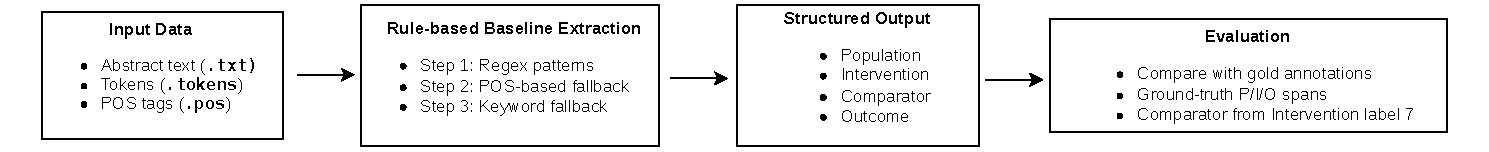
\includegraphics[width=\linewidth]{baseline.drawio.pdf}
    \caption{Overview of the rule-based baseline extraction pipeline. The system uses raw abstract text together with token and POS information, then applies a three-step cascade of regex matching, POS-based fallback, and keyword fallback to produce structured output fields for evaluation.}
    \label{fig:baseline_pipeline}
\end{figure}

For each target field, the baseline system applies a \textbf{three-step priority cascade}. The extraction process starts with the most specific rules and then falls back to more general heuristics if no match is found.

\textbf{Step 1: Regex patterns.}
A set of regular expressions is applied to the raw abstract text in order of specificity, and the first successful match is returned. For example, \textit{Population} extraction first attempts to identify expressions containing a cardinal number followed by a participant-related noun, such as ``200 patients'', before falling back to broader patterns that capture patient-related phrases with nearby context.

\textbf{Step 2: POS-based fallback.}
If no regex pattern matches, the system scans the POS tag sequence for field-specific syntactic patterns. For \textit{Population}, this includes patterns such as a cardinal number tag (\texttt{CD}) followed by a singular or plural noun (\texttt{NN}/\texttt{NNS}). For \textit{Intervention} and \textit{Outcome}, the system identifies trigger verbs and collects the following noun-phrase-like tokens as candidate spans.

\textbf{Step 3: Keyword fallback.}
If both previous steps fail, the system returns a keyword match from a predefined domain vocabulary. For example, \textit{Outcome} extraction falls back to terms such as ``mortality'', ``pain'', or ``blood pressure''.

Table~\ref{tab:baseline_rules} provides representative examples of the main rule types used for each field, rather than an exhaustive list of all implemented patterns.

\begin{table}[ht]
\centering
\small
\begin{tabular}{p{0.16\linewidth} p{0.24\linewidth} p{0.22\linewidth} p{0.24\linewidth}}
\hline
\textbf{Field} & \textbf{Regex (Step 1)} & \textbf{POS (Step 2)} & \textbf{Keyword (Step 3)} \\
\hline
Population & number + participant noun & \texttt{CD} + \texttt{NN}/\texttt{NNS} & patients, subjects \\
Intervention & treatment trigger + following phrase & trigger verb + noun phrase & therapy, treatment \\
Comparator & comparative marker + following phrase & placebo/sham + noun phrase & placebo, control group \\
Outcome & outcome trigger + following phrase & trigger verb + noun phrase & mortality, pain \\
\hline
\end{tabular}
\caption{Representative examples of the main rule types used in the baseline extraction system. The table is illustrative rather than exhaustive.}
\label{tab:baseline_rules}
\end{table}

These examples are intended to illustrate the overall rule design. In practice, each field is handled by a broader set of regex patterns, POS-based heuristics, and fallback keywords.

\subsubsection{Limitations of the Baseline}

The rule-based system outputs only a single span per field, which limits recall when multiple spans are present in the ground truth annotations. In addition, the method is sensitive to wording variation and cannot reliably resolve lexical ambiguity. For example, the conjunction ``or'' may indicate a true comparator relation, as in ``drug A or placebo'', but it may also simply connect related expressions, such as ``efficacy or safety'', leading to false positives in comparator extraction. More generally, because the system depends on handcrafted lexical and syntactic patterns, it may struggle when important information is expressed indirectly, distributed across sentences, or described using wording not covered by the predefined rules.

\subsection{Axes of Experimentation}

To examine how different design choices affect extraction performance, we compared our methods along two main experimental axes. The first axis focuses on the \textbf{extraction approach}, comparing the rule-based baseline with \textbf{LLM-based} strategies such as zero-shot and few-shot prompting. The second axis focuses on \textbf{pipeline design}, comparing \textbf{end-to-end} extraction with a more \textbf{decomposed} multi-step pipeline. Figure~\ref{fig:axes_of_experimentation} summarises these two axes and the main variants explored in our study.

\begin{figure}[ht]
    \centering
    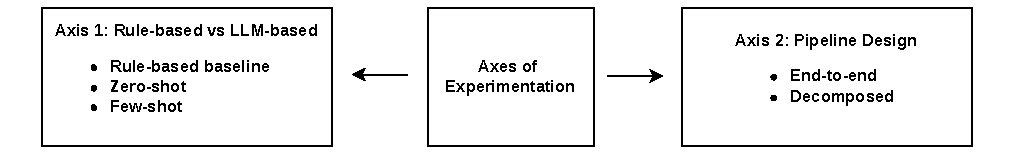
\includegraphics[width=0.85\linewidth]{axisofexperiment.drawio.pdf}
    \caption{Summary of the two experimental axes explored in this study. Axis 1 compares rule-based and LLM-based extraction strategies, while Axis 2 compares end-to-end and decomposed pipeline designs.}
    \label{fig:axes_of_experimentation}
\end{figure}

\subsubsection{Axis 1: Rule-based vs LLM-based Extraction}

The first experimental axis compares \textbf{rule-based} and \textbf{LLM-based} extraction strategies. This axis was chosen to examine the trade-off between explicit handcrafted patterns and more flexible language-model-based extraction. The rule-based baseline relies on regex rules, POS-based heuristics, and keyword matching, which are expected to work well when relevant information is expressed using predictable lexical or syntactic patterns. However, this approach may struggle when the wording is indirect, highly variable, or spread across longer contexts.

\paragraph{Proposed improvements.}
Along this axis, our main proposed improvements are the use of \textbf{zero-shot} and \textbf{few-shot} LLM prompting as alternatives to the rule-based baseline. The zero-shot setting allows the model to extract field information without task-specific examples, while the few-shot setting provides a small number of demonstrations to guide the model towards the intended schema. These approaches are intended to improve extraction coverage by handling broader linguistic variation and by capturing field-relevant information that is not explicitly covered by handcrafted rules. Because large language models are pretrained on large-scale text corpora, they may capture richer semantic and contextual patterns, which could be especially helpful when target information is expressed indirectly or in less predictable forms.

\paragraph{Hypotheses.}
We hypothesise that the \textbf{rule-based baseline} may achieve relatively high precision on clearly structured and lexically predictable abstracts, but may have limited recall when field information is expressed in less regular forms. In contrast, the \textbf{zero-shot LLM} is expected to offer better flexibility and coverage, although its outputs may be less stable or schema-consistent. The \textbf{few-shot LLM} is expected to perform better than zero-shot prompting, since the additional examples should help the model follow the required output structure more closely and distinguish the target fields more consistently.

\section{Experimental evaluation}
\label{headings}


All headings should be lower case (except for first word and proper nouns),
flush left, and bold.


First-level headings should be in 12-point type.


\subsection{Headings: second level}


Second-level headings should be in 10-point type.


\subsubsection{Headings: third level}


Third-level headings should be in 10-point type.


\paragraph{Paragraphs}


There is also a \verb+\paragraph+ command available, which sets the heading in
bold, flush left, and inline with the text, with the heading followed by 1\,em
of space.


\section{Conclusions}
\label{others}


These instructions apply to everyone.


\subsection{Citations within the text}


The \verb+natbib+ package will be loaded for you by default.  Citations may be
author/year or numeric, as long as you maintain internal consistency.  As to the
format of the references themselves, any style is acceptable as long as it is
used consistently.


The documentation for \verb+natbib+ may be found at
\begin{center}
  \url{http://mirrors.ctan.org/macros/latex/contrib/natbib/natnotes.pdf}
\end{center}
Of note is the command \verb+\citet+, which produces citations appropriate for
use in inline text.  For example,
\begin{verbatim}
   \citet{hasselmo} investigated\dots
\end{verbatim}
produces
\begin{quote}
  Hasselmo, et al.\ (1995) investigated\dots
\end{quote}


If you wish to load the \verb+natbib+ package with options, you may add the
following before loading the \verb+neurips_2026+ package:
\begin{verbatim}
   \PassOptionsToPackage{options}{natbib}
\end{verbatim}


If \verb+natbib+ clashes with another package you load, you can add the optional
argument \verb+nonatbib+ when loading the style file:
\begin{verbatim}
   \usepackage[nonatbib]{neurips_2026}
\end{verbatim}


As submission is double blind, refer to your own published work in the third
person. That is, use ``In the previous work of Jones et al.\ [4],'' not ``In our
previous work [4].'' If you cite your other papers that are not widely available
(e.g., a journal paper under review), use anonymous author names in the
citation, e.g., an author of the form ``A.\ Anonymous'' and include a copy of the anonymized paper in the supplementary material.


\subsection{Footnotes}


Footnotes should be used sparingly.  If you do require a footnote, indicate
footnotes with a number\footnote{Sample of the first footnote.} in the
text. Place the footnotes at the bottom of the page on which they appear.
Precede the footnote with a horizontal rule of 2~inches (12~picas).


Note that footnotes are properly typeset \emph{after} punctuation
marks.\footnote{As in this example.}


\subsection{Figures}


\begin{figure}
  \centering
  \fbox{\rule[-.5cm]{0cm}{4cm} \rule[-.5cm]{4cm}{0cm}}
  \caption{Sample figure caption. Explain what the figure shows and add a key take-away message to the caption.}
\end{figure}


All artwork must be neat, clean, and legible. Lines should be dark enough for
 reproduction purposes. The figure number and caption always appear after the
figure. Place one line space before the figure caption and one line space after
the figure. The figure caption should be lower case (except for the first word and proper nouns); figures are numbered consecutively.


You may use color figures.  However, it is best for the figure captions and the
paper body to be legible if the paper is printed in either black/white or in
color.


\subsection{Tables}


All tables must be centered, neat, clean, and legible.  The table number and
title always appear before the table.  See Table~\ref{sample-table}.


Place one line space before the table title, one line space after the
table title, and one line space after the table. The table title must
be lower case (except for the first word and proper nouns); tables are
numbered consecutively.


Note that publication-quality tables \emph{do not contain vertical rules}. We
strongly suggest the use of the \verb+booktabs+ package, which allows for
typesetting high-quality, professional tables:
\begin{center}
  \url{https://www.ctan.org/pkg/booktabs}
\end{center}
This package was used to typeset Table~\ref{sample-table}.


\begin{table}
  \caption{Sample table caption. Explain what the table shows and add a key take-away message to the caption.}
  \label{sample-table}
  \centering
  \begin{tabular}{lll}
    \toprule
    \multicolumn{2}{c}{Part}                   \\
    \cmidrule(r){1-2}
    Name     & Description     & Size ($\mu$m) \\
    \midrule
    Dendrite & Input terminal  & $\approx$100     \\
    Axon     & Output terminal & $\approx$10      \\
    Soma     & Cell body       & up to $10^6$  \\
    \bottomrule
  \end{tabular}
\end{table}

\subsection{Math}
Note that display math in bare TeX commands will not create correct line numbers for submission. Please use LaTeX (or AMSTeX) commands for unnumbered display math. (You really shouldn't be using \$\$ anyway; see \url{https://tex.stackexchange.com/questions/503/why-is-preferable-to} and \url{https://tex.stackexchange.com/questions/40492/what-are-the-differences-between-align-equation-and-displaymath} for more information.)

\subsection{Final instructions}

Do not change any aspects of the formatting parameters in the style files.  In
particular, do not modify the width or length of the rectangle the text should
fit into, and do not change font sizes. Please note that pages should be
numbered.


\section{Preparing PDF files}


Please prepare submission files with paper size ``US Letter,'' and not, for
example, ``A4.''


Fonts were the main cause of problems in the past years. Your PDF file must only
contain Type 1 or Embedded TrueType fonts. Here are a few instructions to
achieve this.


\begin{itemize}


\item You should directly generate PDF files using \verb+pdflatex+.


\item You can check which fonts a PDF files uses.  In Acrobat Reader, select the
  menu Files$>$Document Properties$>$Fonts and select Show All Fonts. You can
  also use the program \verb+pdffonts+ which comes with \verb+xpdf+ and is
  available out-of-the-box on most Linux machines.


\item \verb+xfig+ ``patterned'' shapes are implemented with bitmap fonts.  Use
  "solid" shapes instead.


\item The \verb+\bbold+ package almost always uses bitmap fonts.  You should use
  the equivalent AMS Fonts:
\begin{verbatim}
   \usepackage{amsfonts}
\end{verbatim}
followed by, e.g., \verb+\mathbb{R}+, \verb+\mathbb{N}+, or \verb+\mathbb{C}+
for $\mathbb{R}$, $\mathbb{N}$ or $\mathbb{C}$.  You can also use the following
workaround for reals, natural and complex:
\begin{verbatim}
   \newcommand{\RR}{I\!\!R} %real numbers
   \newcommand{\Nat}{I\!\!N} %natural numbers
   \newcommand{\CC}{I\!\!\!\!C} %complex numbers
\end{verbatim}
Note that \verb+amsfonts+ is automatically loaded by the \verb+amssymb+ package.


\end{itemize}


If your file contains type 3 fonts or non embedded TrueType fonts, we will ask
you to fix it.


\subsection{Margins in \LaTeX{}}


Most of the margin problems come from figures positioned by hand using
\verb+\special+ or other commands. We suggest using the command
\verb+\includegraphics+ from the \verb+graphicx+ package. Always specify the
figure width as a multiple of the line width as in the example below:
\begin{verbatim}
   \usepackage[pdftex]{graphicx} ...
   \includegraphics[width=0.8\linewidth]{myfile.pdf}
\end{verbatim}
See Section 4.4 in the graphics bundle documentation
(\url{http://mirrors.ctan.org/macros/latex/required/graphics/grfguide.pdf})


A number of width problems arise when \LaTeX{} cannot properly hyphenate a
line. Please give LaTeX hyphenation hints using the \verb+\-+ command when
necessary.

\begin{ack}
Use unnumbered first level headings for the acknowledgments. All acknowledgments
go at the end of the paper before the list of references. Moreover, you are required to declare
funding (financial activities supporting the submitted work) and competing interests (related financial activities outside the submitted work).
More information about this disclosure can be found at: \url{https://neurips.cc/Conferences/2026/PaperInformation/FundingDisclosure}.


Do {\bf not} include this section in the anonymized submission, only in the final paper. You can use the \texttt{ack} environment provided in the style file to automatically hide this section in the anonymized submission.
\end{ack}

\section*{References}


References follow the acknowledgments in the camera-ready paper. Use unnumbered first-level heading for
the references. Any choice of citation style is acceptable as long as you are
consistent. It is permissible to reduce the font size to \verb+small+ (9 point)
when listing the references.
Note that the Reference section does not count towards the page limit.
\medskip


{
\small


[1] Alexander, J.A.\ \& Mozer, M.C.\ (1995) Template-based algorithms for
connectionist rule extraction. In G.\ Tesauro, D.S.\ Touretzky and T.K.\ Leen
(eds.), {\it Advances in Neural Information Processing Systems 7},
pp.\ 609--616. Cambridge, MA: MIT Press.


[2] Bower, J.M.\ \& Beeman, D.\ (1995) {\it The Book of GENESIS: Exploring
  Realistic Neural Models with the GEneral NEural SImulation System.}  New York:
TELOS/Springer--Verlag.


[3] Hasselmo, M.E., Schnell, E.\ \& Barkai, E.\ (1995) Dynamics of learning and
recall at excitatory recurrent synapses and cholinergic modulation in rat
hippocampal region CA3. {\it Journal of Neuroscience} {\bf 15}(7):5249-5262.
}


%%%%%%%%%%%%%%%%%%%%%%%%%%%%%%%%%%%%%%%%%%%%%%%%%%%%%%%%%%%%

\appendix

\section{Technical appendices and supplementary material}
Technical appendices with additional results, figures, graphs, and proofs may be submitted with the paper submission before the full submission deadline (see above). You can upload a ZIP file for videos or code, but do not upload a separate PDF file for the appendix. There is no page limit for the technical appendices. 

Note: Think of the appendix as ``optional reading'' for reviewers. The paper must be able to stand alone without the appendix; for example, adding critical experiments that support the main claims to an appendix is inappropriate. 

%%%%%%%%%%%%%%%%%%%%%%%%%%%%%%%%%%%%%%%%%%%%%%%%%%%%%%%%%%%%

\newpage
\input{checklist.tex}


\end{document}